\subsection{Moduł zarządzający komunikacją z klientem}
\label{sec:comminicator}
Moduł \textit{communicator} zarządza procesem komunikacji z klientem oraz kontroli poprawności przesyłanych danych. Zadaniem modułu jest realizacja serwerowej części ustalonego protokołu komunikacji z klientem (rozdz. \ref{sec:przebieg-komunikacji}), w szczególności:
\begin{itemize}[noitemsep, nolistsep]
\item zarządzanie procesem przesyłania bloków i potwierdzeń
\item kontrola poprawności bloków
\item obsługa retransmisji niepoprawnych bloków
\item odebranie klucza szyfrującego, wektora inicjalizacji oraz informacji, czy bloki powinny być szyfrowane, czy deszyfrowane
\item zarządzanie procesem szyfrowania, w tym za łączenie bloków zgodnie ze standardem CBC.
\end{itemize}

\begin{figure}[!h]
\begin{lstlisting}[style=vhdl, captionpos=b, caption={\textit{communicator} -- interfejs modułu}]
port (
	clk_16  : in    std_logic;
	reset_n : in    std_logic;
	rx      : in    std_logic;
	tx      : out   std_logic);
\end{lstlisting}
\end{figure}

Opis sygnałów interfejsu modułu \textit{communicator}:
\begin{interface}{CLK\_16}
	\item[\insignal{CLK\_16}] główny zegar układu.
	\item[\insignal{RX}] zsynchronizowany z zegarem \insignal{CLK\_16} sygnał UART RX wychodzący do układu konwertera USB-UART.
	\item[\outsignal{TX}] sygnał UART TX pochodzący z układu konwertera USB-UART.
\end{interface}

Główną częścią modułu \textit{communicator} jest maszyna stanów sterująca wszystkimi realizowanymi zadaniami. Moduł zawiera również instancję innych zdefiniowanych komponentów, które dostarczają niezbędnych funkcjonalności. Na schemacie modułu (rys. \ref{fig:communicator-schemat}) sygnały po lewej stronie wychodzą z maszyny stanów, a sygnały po prawej stronie stanowią jej wejścia. Wyjątkami są sygnały \insignal{RX} i \outsignal{TX}, które są interfejsem modułu i nie są bezpośrednio podłączone do maszyny. Schemat nie zawiera wszystkich sygnałów pojawiających się w implementacji. Pominięte zostały sygnały pomocnicze, które nie są niezbędne do zrozumienia działania układu. Również główny zegar nie został przedstawiony, jest on podłączony do wszystkich modułów poza \textit{key\_expansion}, \textit{aes\_enc}, \textit{aes\_dec}.

Rysunki \ref{fig:communicator-state-machine-1} oraz \ref{fig:communicator-state-machine-2} przedstawiają wszystkie stany maszyny wraz z pseudokodem wykonywanych w nich operacji. Maszyna stanów jest taktowana głównym zegarem \insignal{CLK\_16}, podczas każdego zbocza rosnącego wykonywany jest kod wewnątrz aktywnego stanu. Instrukcje pseudokodu to:
\begin{description}[noitemsep]
	\item[\textbf{state \textit{x}}] -- przejście do stanu \textit{x}.
	\item[\textbf{mux \textit{x}}] -- ustawienie odpowiedniego sygnału, w taki sposób aby selektory byte/block lub enc/dec znalazły się w odpowiednim stanie.
	\item[\textbf{trigger \textit{x}}] -- ustawienie sygnału \textit{x} w stan wysoki na 1 okres głównego zegara zaczynając od kolejnego zbocza malejącego 
	\item[\textbf{store \textit{x} into \textit{y}}] -- ustawienie sygnału \textit{y} na wartość \textit{x}
\end{description}

%%%%%%%%%%%%%%%%%%%%%%%%%%%%%%%%%%%%%%%%%%%%%%%%%%%%%%%%%%%%%%%%%%%%%%%%%%%%%%%%%%%%%%%%%%%%%%%%%%%%%%%%
%%%%%%%%%%%%%%%%%%%%%%%%%%%%%%%%%%%%%%%%%%%%%%%%%%%%%%%%%%%%%%%%%%%%%%%%%%%%%%%%%%%%%%%%%%%%%%%%%%%%%%%%
%%%%%%%%%%%%%%%%%%%%%%%%%%%%%%%%%%%%%%%%%%%%%%%%%%%%%%%%%%%%%%%%%%%%%%%%%%%%%%%%%%%%%%%%%%%%%%%%%%%%%%%%
\tikzset{
    state/.style={
           rectangle,
           rounded corners,
           draw=black, very thick,
           minimum height=2em,
           inner sep=2pt,
           text centered,
           },
}

\begin{figure}
\centering
\begin{tikzpicture}[->,>=stealth', y=-1cm]

\node[state, initial] (start) {
\begin{tabular}{l}
	\textbf{start}\\
	\begin{lstlisting}[language=Python, basicstyle=\tiny\ttfamily, autogobble=true,
    tabsize=3, morekeywords={state, trigger, mux}]
		mux byte
		trigger byte_receive
		state choice
	\end{lstlisting}
\end{tabular}
};

\node[state, below=of start] (choice) {
\begin{tabular}{l}
	\textbf{choice}\\
	\begin{lstlisting}[language=Python, basicstyle=\tiny\ttfamily, autogobble=true,
    tabsize=3, morekeywords={state, trigger, mux, store, into}]
		if finished_byte_receive
			if byte_received == ENC:
				mux aes_enc
				store ACK into byte_to_send
			elif byte_received == DEC:
				mux aes_dec
				store ACK into byte_to_send
			else:
				store NACK into byte_to_send	
		
			trigger send_byte
			state choice_ack
	\end{lstlisting}
\end{tabular}
};

\node[state, right=of choice] (choice_ack) {
\begin{tabular}{l}
	\textbf{choice\_ack}\\
	\begin{lstlisting}[language=Python, basicstyle=\tiny\ttfamily, autogobble=true,
    tabsize=3, morekeywords={state, trigger, mux}]
		if finished_byte_send 
			if byte_to_send == ACK:
				mux block
				trigger block_receive
				state key_low
			else:
				trigger byte_receive
				state choice
	\end{lstlisting}
\end{tabular}
};

\node[state, below=of choice] (key_low) {
\begin{tabular}{l}
	\textbf{key\_low}\\
	\begin{lstlisting}[language=Python, basicstyle=\tiny\ttfamily, autogobble=true,
    tabsize=3, morekeywords={state, trigger, state, store, into, mux}]
		if finished_block_receive 
			if crc_correct:
				store block_received into key_low
				store ACK into byte_to_send
			else:
				store NACK into byte_to_send
	
			mux byte
			trigger byte_send
			state key_low_ack
	\end{lstlisting}
\end{tabular}
};

\node[state, right=of key_low] (key_low_ack) {
\begin{tabular}{l}
	\textbf{key\_low\_ack}\\
	\begin{lstlisting}[language=Python, basicstyle=\tiny\ttfamily, autogobble=true,
    tabsize=3, morekeywords={state, trigger, mux}]
		if finished_byte_send:
			if byte_sent == ACK:
				state key_high
			else:
				state key_low
		
			mux block
			trigger block_receive
	\end{lstlisting}
\end{tabular}
};

\node[state, below=of key_low] (key_high) {
\begin{tabular}{l}
	\textbf{key\_high}\\
	\begin{lstlisting}[language=Python, basicstyle=\tiny\ttfamily, autogobble=true,
    tabsize=3, morekeywords={state, trigger, state, store, into, mux}]
		if finished_block_receive:
			if crc_correct:
				store block_received into key_high
				store ACK into byte_to_send
			elif finished_block_receive:
				store NACK into byte_to_send
	
			mux byte
			trigger byte_send
			state key_high_ack
	\end{lstlisting}
\end{tabular}
};

\node[state, right=of key_high] (key_high_ack) {
\begin{tabular}{l}
	\textbf{key\_high\_ack}\\
	\begin{lstlisting}[language=Python, basicstyle=\tiny\ttfamily, autogobble=true,
    tabsize=3, morekeywords={state, trigger, mux}]
		if finished_byte_send:
			if byte_sent == ACK:
				state init_vector
			else:
				state key_high

			mux block
			trigger block_receive
	\end{lstlisting}
\end{tabular}
};

\node[state, below=of key_high] (init_vector) {
\begin{tabular}{l}
	\textbf{init\_vector}\\
	\begin{lstlisting}[language=Python, basicstyle=\tiny\ttfamily, autogobble=true,
    tabsize=3, morekeywords={state, trigger, mux, store, into}]
		if finished_block_receive 
			if crc_correct:
				store block_received into aes_enc_prev_ciphertext
				store block_received into aes_dec_prev_ciphertext
				store ACK into byte_to_send
			else:
				store NACK into byte_to_send

			mux byte
			trigger byte_send
			state init_vector_ack
	\end{lstlisting}
\end{tabular}
};

\node[state, right=of init_vector] (init_vector_ack) {
\begin{tabular}{l}
	\textbf{init\_vector\_ack}\\
	\begin{lstlisting}[language=Python, basicstyle=\tiny\ttfamily, autogobble=true,
    tabsize=3, morekeywords={state, trigger, mux}]
		if finished_byte_send
			if byte_sent == ACK:
				state first_block
			else:
				state init_vector	

			mux block
			trigger block_receive
	\end{lstlisting}
\end{tabular}
};


\node[state, below=of init_vector_ack] (first_block) {
\begin{tabular}{l}
	\textbf{first\_block}
\end{tabular}
};

\path[->] (start) edge node {} (choice);

\path[->] (choice) edge node {} (choice_ack);
\path[->] (choice_ack) edge node {} (key_low);
\path[->] (choice_ack) edge [bend right] node {} (choice);

\path[->] (key_low) edge node {} (key_low_ack);
\path[->] (key_low_ack) edge node {} (key_high);
\path[->] (key_low_ack) edge [bend right] node {} (key_low);

\path[->] (key_high) edge node {} (key_high_ack);
\path[->] (key_high_ack) edge node {} (init_vector);
\path[->] (key_high_ack) edge [bend right] node {} (key_high);

\path[->] (init_vector) edge node {} (init_vector_ack);
\path[->] (init_vector_ack) edge node {} (first_block);
\path[->] (init_vector_ack) edge [bend right] node {} (init_vector);

\end{tikzpicture}
\caption{Maszyna stanów modułu \textit{communicator} -- stany początkowe}
\label{fig:communicator-state-machine-1}
\end{figure}


%%%%%%%%%%%%%%%%%%%%%%%%%%%%%%%%%%%%%%%%%%%%%%%%%%%%%%%%%%%%%%%%%%%%%%%%%%%%%%%%%%%%%%%%%%%%%%%%%%%%%%%%
%%%%%%%%%%%%%%%%%%%%%%%%%%%%%%%%%%%%%%%%%%%%%%%%%%%%%%%%%%%%%%%%%%%%%%%%%%%%%%%%%%%%%%%%%%%%%%%%%%%%%%%%
%%%%%%%%%%%%%%%%%%%%%%%%%%%%%%%%%%%%%%%%%%%%%%%%%%%%%%%%%%%%%%%%%%%%%%%%%%%%%%%%%%%%%%%%%%%%%%%%%%%%%%%%

\begin{figure}
\centering
\begin{tikzpicture}[->,>=stealth', y=-1cm]

\node[state] (first_block) {
\begin{tabular}{l}
	\textbf{first\_block}\\
	\begin{lstlisting}[language=Python, basicstyle=\tiny\ttfamily, autogobble=true,
    tabsize=3, morekeywords={state, trigger, store, into, mux}]
		if finished_block_receive:
			if crc_correct:
				store block_received into maybe_next_block_to_send
				store ACK into byte_to_send
			else:
				store NACK into byte_to_send

			mux byte
			trigger byte_send
			trigger byte_receive
			state blocks_ack
	\end{lstlisting}
\end{tabular}
};

\node[state, below=0.7cm of first_block] (blocks) {
\begin{tabular}{l}
	\textbf{blocks}\\
	\begin{lstlisting}[language=Python, basicstyle=\tiny\ttfamily, autogobble=true,
    tabsize=3, morekeywords={state, trigger, store, into, mux}]
		if finished_block_receive and finished_block_send:
			# send and receive finished simultaneously
			if crc_correct:
				store block_received into maybe_next_block_to_send
				store aes_enc_ciphertext into aes_enc_prev_ciphertext
				store aes_dec_ciphertext into aes_dec_prev_ciphertext
				store ACK into byte_to_send
			else:
				store NACK into byte_to_send

			mux byte
			trigger byte_send
			trigger byte_receive
			state blocks_ack

		elif finished_block_receive:
			# receive finished first
			if crc_correct:
				store block_received into maybe_next_block_to_send
				store aes_enc_ciphertext into aes_enc_prev_ciphertext
				store aes_dec_ciphertext into aes_dec_prev_ciphertext
				store ACK into byte_to_send
			else:
				store NACK into byte_to_send
				
			state blocks_r_finished_t_waiting

		elif finished_block_send:
			# send finished first
			state blocks_r_waiting_t_finished
	\end{lstlisting}
\end{tabular}
};

\node[state, above right= -1cm and 2.5cm of first_block] (blocks_r_finished_t_waiting) {
\begin{tabular}{l}
	\textbf{blocks\_r\_finished\_t\_waiting}\\
	\begin{lstlisting}[language=Python, basicstyle=\tiny\ttfamily, autogobble=true,
    tabsize=3, morekeywords={state, trigger, mux}]
    	if finished_block_send:
    		mux byte
    		trigger byte_send
    		trigger byte_receive
    		state blocks_ack
	\end{lstlisting}
\end{tabular}
};

\node[state, below=0.7cm of blocks_r_finished_t_waiting] (blocks_r_waiting_t_finished) {
\begin{tabular}{l}
	\textbf{blocks\_r\_waiting\_t\_finished}\\
	\begin{lstlisting}[language=Python, basicstyle=\tiny\ttfamily, autogobble=true,
    tabsize=3, morekeywords={state, trigger, store, into, mux}]
		if finished_block_receive:
			if crc_correct:
				store block_received into maybe_next_block_to_send
				store aes_enc_ciphertext into aes_enc_prev_ciphertext
				store aes_dec_ciphertext into aes_dec_prev_ciphertext
				store ACK into byte_to_send
			else:
				store NACK into byte_to_send

			mux byte
			trigger byte_send
			trigger byte_receive
			state blocks_ack
	\end{lstlisting}
\end{tabular}
};

\node[state, below=0.7cm of blocks_r_waiting_t_finished] (blocks_ack) {
\begin{tabular}{l}
	\textbf{blocks\_ack}\\
	\begin{lstlisting}[language=Python, basicstyle=\tiny\ttfamily, autogobble=true,
    tabsize=3, morekeywords={state, trigger, store, into, mux}]
		if finished_byte_receive and finished_byte_send:
			# send and receive finished simultaneously 
			if byte_received == FIN:
				if byte_to_send == ACK:
					store maybe_next_block_to_send into block_to_send
				state finishing
			elif byte_received == ACK:			
				if byte_to_send == ACK:
					store maybe_next_block_to_send into block_to_send
				trigger block_receive	
				state blocks
			else:			
				trigger block_receive
				state blocks

			mux block
			trigger block_send

		elif finished_byte_receive:
			# receive finished first
			if byte_received == FIN:
				store True into finished
				if byte_to_send == ACK:
					store maybe_next_block_to_send into block_to_send
			elif byte_received == ACK:			
				store False into finished
				if byte_to_send == ACK:
					store maybe_next_block_to_send into block_to_send
			else:			
				store False into finished

			state acks_r_finished_t_waiting

		elif finished_bytev_send:
			# send finished first
			state acks_r_waiting_t_finished

	\end{lstlisting}
\end{tabular}
};

\node[state, below=0.7cm of blocks] (acks_r_finished_t_waiting) {
\begin{tabular}{l}
	\textbf{acks\_r\_finished\_t\_waiting}\\
	\begin{lstlisting}[language=Python, basicstyle=\tiny\ttfamily, autogobble=true,
    tabsize=3, morekeywords={state, trigger, mux}]
		if finished_byte_send:
			if finished:
				state finishing
			else:
				trigger block_receive
				state blocks

			mux block
			trigger block_send

	\end{lstlisting}
\end{tabular}
};

\node[state, below=0.7cm of acks_r_finished_t_waiting] (acks_r_waiting_t_finished) {
\begin{tabular}{l}
	\textbf{acks\_r\_waiting\_t\_finished}\\
	\begin{lstlisting}[language=Python, basicstyle=\tiny\ttfamily, autogobble=true,
    tabsize=3, morekeywords={state, trigger, store, into, mux}]
		if finished_block_receive:
			if byte_received == FIN:
				if byte_to_send == ACK:
					store maybe_next_block_to_send into block_to_send
				state finishing
			elif byte_received == ACK:			
				if byte_to_send == ACK:
					store maybe_next_block_to_send into block_to_send
				trigger block_receive	
				state blocks
			else:			
				trigger block_receive
				state blocks

			mux block
			trigger block_send
	\end{lstlisting}
\end{tabular}
};

\node[state, below=0.7cm of blocks_ack] (finishing) {
\begin{tabular}{l}
	\textbf{finishing}\\
	\begin{lstlisting}[language=Python, basicstyle=\tiny\ttfamily, autogobble=true,
    tabsize=3, morekeywords={state, trigger, mux}]
		if finished_block_send:
			mux block
			trigger byte_receive
			state finishing_ack
	
	\end{lstlisting}
\end{tabular}
};

\node[state, below=0.7cm of finishing] (finishing_ack) {
\begin{tabular}{l}
	\textbf{finishing\_ack}\\
	\begin{lstlisting}[language=Python, basicstyle=\tiny\ttfamily, autogobble=true,
    tabsize=3, morekeywords={state, trigger, mux}]
		if finished_byte_receive:
			if byte_receive == ACK or byte_received == FIN:
				trigger byte_receive
				state choice
			else:
				mux block
				trigger block_receive
				state finishing
	
	\end{lstlisting}
\end{tabular}
};

\node[state, above=0.7cm of first_block] (init_vector_ack) {
\begin{tabular}{l}
	\textbf{init\_vector\_ack}
\end{tabular}
};

\node[state, below=0.7cm of finishing_ack] (choice) {
\begin{tabular}{l}
	\textbf{choice}
\end{tabular}
};

\path[->] (init_vector_ack) edge node {} (first_block);

% \path[->] (first_block) edge node {} (blocks_ack);
\draw[->] let \p{MIDX}=($(blocks.east)!0.33!(blocks_r_waiting_t_finished.west)$) in
          let \p{MIDY}=($(first_block.south)!0.5!(blocks.north)$) in
          let \p{DESTY}=($(blocks.east) - (0, 1)$) in
          let \p{A} = ($(first_block.south -| first_block.east) - (0, 0.5)$) in
          (\p{A}) -- (\x{MIDX}, \y{A}) -- (\x{MIDX}, \y{DESTY}) -- (\p{DESTY} -| blocks_ack.west);

% \path[->] (blocks) edge node {} (blocks_ack);
\draw[->] (blocks.east) -- (blocks.east -| blocks_ack.west);

% \path[->] (blocks) edge node {} (blocks_r_finished_t_waiting);
\draw[->] let \p{MIDY}=($(blocks_r_waiting_t_finished.south)!0.66!(blocks.north)$) in
          let \p{MIDX}=($(blocks.east)!0.66!(blocks_r_waiting_t_finished.west)$) in
             (\p{MIDY} -| blocks.east) 
          -- (\p{MIDX} |- \p{MIDY}) 
          -- (\p{MIDX} |- blocks_r_finished_t_waiting.west) 
          -- (blocks_r_finished_t_waiting.west);

% \path[->] (blocks) edge node {} (blocks_r_waiting_t_finished);
\draw[->] let \p{MID}=($(blocks_r_waiting_t_finished.south)!0.33!(blocks.north)$) in
          (\p{MID} -| blocks.east) -- (\p{MID} -| blocks_r_waiting_t_finished.west);

% \path[->] (blocks_r_finished_t_waiting) edge node {} (blocks_ack);
\draw[->] let \p{A}=($(blocks_r_finished_t_waiting.east) + (2, 0)$) in
          let \p{B}=(blocks_ack.east) in
			 (blocks_r_finished_t_waiting.east) 
    	  -- (\x{A}, \y{A})
    	  -- (\x{A}, \y{B})
    	  -- (blocks_ack.east);

\path[->] (blocks_r_waiting_t_finished) edge node {} (blocks_ack);

% \path[->] (blocks_ack) edge node {} (blocks);
\draw[->] let \p{A}=($(blocks.east) + (0, 1)$) in 
          (\p{A} -| blocks_ack.west) -- (\p{A});

\path[->] (blocks_ack) edge node {} (finishing);

% \path[->] (blocks_ack) edge node {} (acks_r_finished_t_waiting);
\draw[->] let \p{A}=($(acks_r_finished_t_waiting.north -| acks_r_finished_t_waiting.east) + (0, 0.7)$) in
          (\p{A} -| blocks_ack.west) -- (\p{A});

% \path[->] (blocks_ack) edge node {} (acks_r_waiting_t_finished);
\draw[->] let \p{A}=($(blocks_ack.south -| blocks_ack.west) - (0, 0.7)$) in
          let \p{B}=($(acks_r_waiting_t_finished.north -| acks_r_waiting_t_finished.east) - (0.7, 0)$) in
          (\p{A}) -- (\p{A} -| \p{B}) -- (\p{B});

\path[->] (acks_r_finished_t_waiting) edge node {} (blocks);

% \path[->] (acks_r_finished_t_waiting) edge node {} (finishing);
\draw[->] let \p{MID}=($(acks_r_finished_t_waiting.south)!0.5!(finishing.north)$) in
		  let \p{A}=($(acks_r_finished_t_waiting.south -| acks_r_finished_t_waiting.east) - (0.5, 0)$) in
          let \p{B}=($(finishing.north -| finishing.west) + (0.5, 0)$) in
          (\p{A}) -- (\p{A} |- \p{MID}) -- (\p{B} |- \p{MID}) -- (\p{B});


% \path[->] (acks_r_waiting_t_finished) edge node {} (blocks);
\draw[->] let \p{MID}=($(blocks.west)!0.5!(acks_r_finished_t_waiting.west)$) in
          (\p{MID} |- acks_r_waiting_t_finished.north) -- (\p{MID} |- blocks.south);


% \path[->] (acks_r_waiting_t_finished) edge node {} (finishing);
\draw[->] (acks_r_waiting_t_finished.east |- finishing.west) -- (finishing.west);

% \path[->] (finishing) edge [bend right] node {} (finishing_ack);
\draw[->] let \p{A}=($(finishing.south) + (0.5, 0)$) in (\p{A}) -- (\p{A} |- finishing_ack.north);

\path[->] (finishing_ack) edge node {} (choice);

% \path[->] (finishing_ack) edge [bend right] node {} (finishing);
\draw[->] let \p{A}=($(finishing.south) - (0.5, 0)$) in (\p{A} |- finishing_ack.north) -- (\p{A});

\end{tikzpicture}
\caption{Maszyna stanów modułu \textit{communicator} -- wymiana bloków danych}
\label{fig:communicator-state-machine-2}
\end{figure}

%%%%%%%%%%%%%%%%%%%%%%%%%%%%%%%%%%%%%%%%%%%%%%%%%%%%%%%%%%%%%%%%%%%%%%%%%%%%%%%%%%%%%%%%%%%%%%%%%%%%%%%%
%%%%%%%%%%%%%%%%%%%%%%%%%%%%%%%%%%%%%%%%%%%%%%%%%%%%%%%%%%%%%%%%%%%%%%%%%%%%%%%%%%%%%%%%%%%%%%%%%%%%%%%%
%%%%%%%%%%%%%%%%%%%%%%%%%%%%%%%%%%%%%%%%%%%%%%%%%%%%%%%%%%%%%%%%%%%%%%%%%%%%%%%%%%%%%%%%%%%%%%%%%%%%%%%%

\begin{figure}
\centering
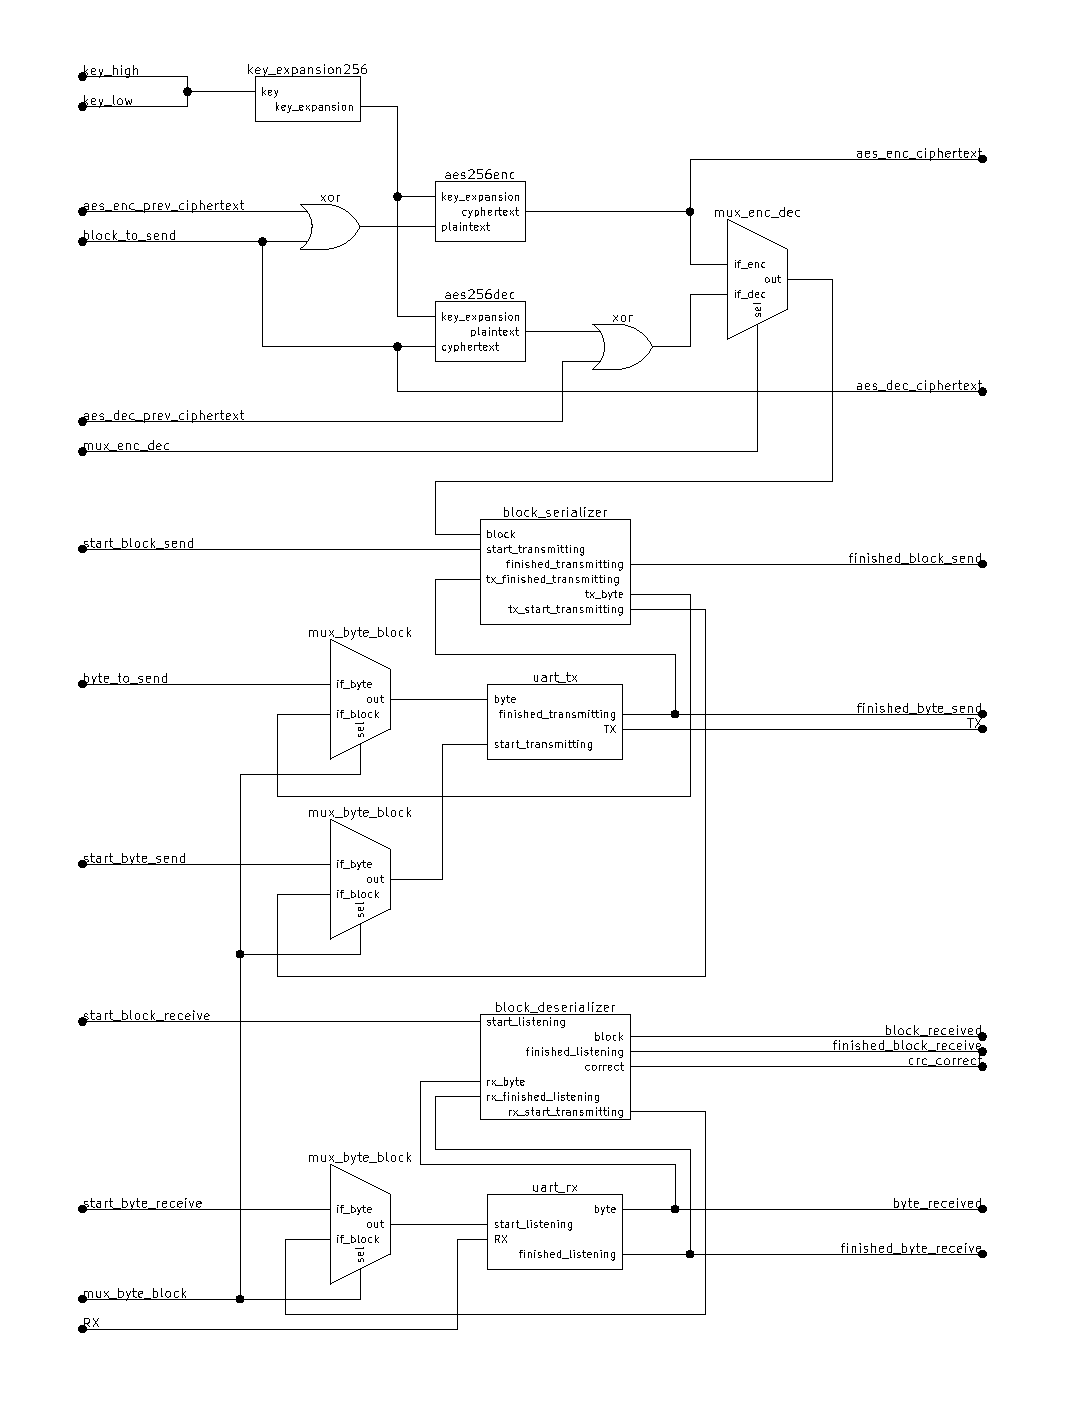
\includegraphics{pictures/communicator.pdf}
\caption{Schemat modułu \textit{communicator}}
\label{fig:communicator-schemat}
\end{figure}

%%%%%%%%%%%%%%%%%%%%%%%%%%%%%%%%%%%%%%%%%%%%%%%%%%%%%%%%%%%%%%%%%%%%%%%%%%%%%%%%%%%%%%%%%%%%%%%%%%%%%%%%
%%%%%%%%%%%%%%%%%%%%%%%%%%%%%%%%%%%%%%%%%%%%%%%%%%%%%%%%%%%%%%%%%%%%%%%%%%%%%%%%%%%%%%%%%%%%%%%%%%%%%%%%
%%%%%%%%%%%%%%%%%%%%%%%%%%%%%%%%%%%%%%%%%%%%%%%%%%%%%%%%%%%%%%%%%%%%%%%%%%%%%%%%%%%%%%%%%%%%%%%%%%%%%%%%

